\documentclass[a4paper,11pt]{article}
\usepackage{setspace}
\onehalfspacing
 
\usepackage{titlesec}
\usepackage{graphicx}
\usepackage{listings}
\usepackage{xcolor}
\usepackage{fancyhdr}
\usepackage[a4paper,margin=1in]{geometry}
\usepackage{mdframed} %nice frames

\definecolor{light-gray}{gray}{0.95} %the shade of grey that stack exchange uses

\renewcommand{\thispagestyle}[1]{} % do nothing

\lstset{
  language=Python,
  aboveskip=3mm,
  belowskip=3mm,
  showstringspaces=true,
  columns=flexible,
  basicstyle={\small\ttfamily},
  numbers=none,
  numberstyle=\tiny\color{gray},
  keywordstyle=\color{blue},
  commentstyle=\color{red},
  breaklines=true,
  breakatwhitespace=true,
  tabsize=2
}

\graphicspath{ {./images/} }
\titlespacing{\section}{0pc}{1pc}{1pc}
 
\pagestyle{fancy}
\fancyhf{}
\rhead{Assignment 5}
\lhead{Internet Traffic Analysis using Wireshark}
\rfoot{Page \thepage}

 
\begin{document}
\title{\vspace{-1.0cm}\textbf{Internet Traffic Analysis using Wireshark}}
\author{
  \textbf{Tan Wei Xuan (49003140)}\\
  \texttt{tanweixuan@postech.ac.kr}
}
\date{\today}
\maketitle

\section{Project Overview}
\textit{\textbf{Wireshark 3.0.1}} is used to analyze the network traffic captured over a specified period of time.

\section{Capturing Packets using Wireshark}

\section{Traffic Analysis using Wireshark}
Analysis is done on the captured network traffic within the provided tracefile. Network period is captured for a period of \textbf{59.088} seconds.

\subsection{Total Number of Packets and Bytes}
\begin{figure}[h!]
	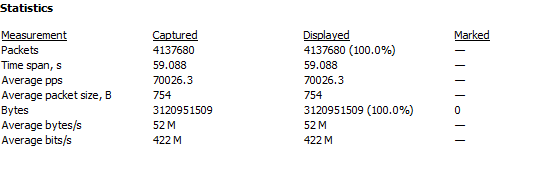
\includegraphics{TtlNoPacketsBytes}
	\caption{\textit{Statistics $\rightarrow$ Capture File Properties}}
\end{figure}
The total number of packets being captured between a \textbf{59 second period} is \textbf{4137680}. The total number of Bytes between captured is \textbf{3120951509}. This information can be obtained thorugh \textit{Stastics $\rightarrow$ Capture File Properties}.

\subsection{Time Difference between First and Last Packet }
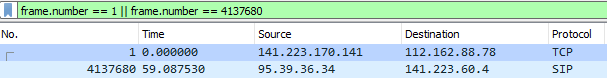
\includegraphics{TimeDiff}
\newline
\newline
We know that the total number of packets being captured is \textbf{4137680}. As such, the first frame be captured will be \textbf{1} and the last frame being captured will be \textbf{4137680}. We can filter out these two frames by applying the filter, \textit{\textbf{(frame.number $==$ 1) $||$ (frame.number $==$ 4137680)}}. From the filtered results, we can see that the first packet is being transmitted at \textbf{0.0} seconds while the last packet is being transmitted at \textbf{59.087530} seconds. As such, the \textbf{time difference} between the \textbf{first} and \textbf{last} packet is \textbf{59.087530 seconds}

\subsection{The number of packet and total bytes of TCP, UDP and ICMP traffic }
\begin{figure}[h!]
	\includegraphics[width = 16cm]{Traffic}
	\caption{\textit{Statistics $\rightarrow$ Protocol Hierarchy}}
\end{figure}
The entirety of the network traffic is being transmitted through \textbf{IPv4} as it takes up \textbf{100\%} of the total packets.
The total number of packet and total bytes of IPv4 TCP, UDP and Internel Control Message Protocol (ICMP) traffic are as follow:
\begin{enumerate}
	\item \textbf{TCP}
	\newline
	The total number of packets being transmitted using TCP is \textbf{1568769} and  the total number of bytes being transmitted is \textbf{43878139}.
	TCP takes up \textbf{37.9\%} of total network traffic.
	\item \textbf{UDP}
	\newline
	The total number of packets being transmitted using UDP is \textbf{2533291} and  the total number of bytes being transmitted is \textbf{20266328}. 	
	UDP takes up \textbf{61.2\%} of total network traffic.
	\item \textbf{ICMP}
	\newline
	The total number of packets being transmitted using ICMP is \textbf{31256} and  the total number of bytes being transmitted is \textbf{978571}. 	
	ICMP takes up \textbf{0.8\%} of total network traffic.
\end{enumerate}
For this captured netwrok traffic, IPv4 TCP and UDP take the majority of the percent of total packets, with \textbf{UDP taking up most of the traffic \textit{(61\%)}}.
This information can be obtained thorugh \textit{Statistics $\rightarrow$ Protocol Hierarchy}.



\subsection{Total Number of Packets and Bytes of each end host}

\subsection{The number of packet and total bytes of FTP, SSH, DNS,  and HTTP}
\subsection{Select  two  applications  other  than  the  aforementioned  applications,  and  print  out  the  number  of packets and the bytes of the traffic which allocates well-known  port  number  (TCP/UDP 1 - 1024) }
\subsection{Enumerate the average packet size, average packet inter-arrival time }


\end{document}